\begin{center}
\hfill \break
\large{МИНИСТЕРСТВО НАУКИ И ВЫСШЕГО ОБРАЗОВАНИЯ РОССИЙСКОЙ ФЕДЕРАЦИИ}\\
\footnotesize{Федеральное государственное автономное образовательное учреждение высшего образования}\\ 
\footnotesize{«Дальневосточный федеральный университет»}\\
\small{\textbf{(ДВФУ)}}\\
\hfill \break
\normalsize{ИНСТИТУТ МАТЕМАТИКИ И КОМПЬЮТЕРНЫХ ТЕХНОЛОГИЙ}\\
 \hfill \break
\normalsize{Департамент математического и компьютерного моделирования}\\
\hfill\break
\hfill \break
\hfill \break
\hfill \break
\large{Алгоритм Форчуна}\\
\hfill \break
\hfill \break
\hfill \break
\normalsize{Доклад\\
\hfill \break
Направление подготовки 09.03.03 Прикладная информатика\\
\hfill \break
Профиль «Приладная информатика в компьютерном дизайне»}\\
\hfill \break
\hfill \break
\end{center}
 
\normalsize{} \hfill \break
\hfill \break
 
\normalsize{ 
\begin{tabular}{cccc}
Обучающийся & \underline{\hspace{3cm}} & &А.В. Быкова \\\\
Руководитель & \underline{\hspace{3cm}}& доцент ИМКТ &А.С. Кленин \\\\
\end{tabular}
}\\
\hfill \break
\hfill \break
\begin{center} Владивосток 2022 \end{center}
\thispagestyle{empty} 
 
\newpage
     
    \tableofcontents 
\newpage


\section{Введение}

\subsection{Диаграмма Вороного}
Формально, диаграмма Вороного это $P = \lbrace p_1,p_2,...,p_n \rbrace $ — множество точек на плоскости.
Если говорить о ее сути, диаграмма Вороного конечного множества точек P на плоскости представляет собой такое разбиение плоскости, при котором каждая область этого разбиения образует множество точек, более близких к одному из элементов множества P, чем к любому другому элементу множества. [10, 11]
Она имеет вид:\\
\begin{figure}[H]
\centering
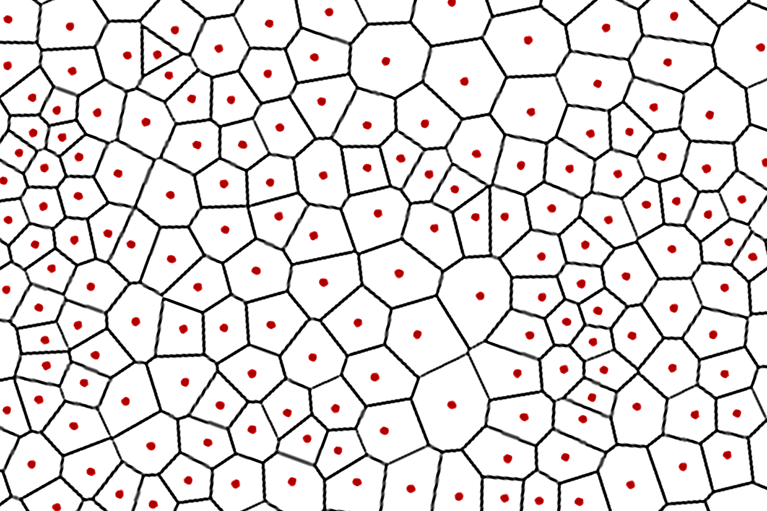
\includegraphics[scale = 0.4]{voronoi}
\caption{\label{tab:widgets}Диаграмма Вороного}
\end{figure}

\subsection{Алгоритм Форчуна}
Для генерации диаграммы Вороного существует Алгоритм Форчуна. Этот алгоритм использует принцип «заметающей прямой». Алгоритм вводит из файла множесто 2D-точек.  Для каждой входной точки, которая называется «сайтом», алгоритм находит область плоскости, все точки которой ближе к этому сайту, чем ко всем остальным.[17, 18] Алгорит Форчуна строит диаграмму Вороного за время O(n log n) с использованием памяти O(n). [6]

\subsection{Авторство}
Данный алгоритм был опубликован Стивеном Форчуном в 1986 году в Нью Джерси во время Второго ежегодного симпозиума по Компьютерной Геометрии. Статья носит название «A Sweepline Algorithm for Voronoi Diagrams» . Название алгоритма происходит от имени его создателя.[9, 14]

\subsection{История развития}
Алгоритм увидел свет в 1986 году, в статье математика Стивена Форчуна под названием «Алгоритм развертки линий для диаграмм Вороного».  На момент своего появления, алгоритм Форчуна был первым в своем роде, который строил диаграмму Вороного с использованием заметающей прямой. [21] Поскольку информация об этом алгоритме, его предшественниках и авторе ограничена, можно сделать вывод, что он не сыскал популярности в свое время. Возможно это произошло из-за сложности вычислений, а может и совсем по другим причинам.[23, 24]

\subsection{Области применения}
Алгоритм используется для построения диаграммы Вороного, которая в свою очередь имеет широкий спектр применения. 
Диаграммы Вороного постоянно использовались антропологами для описания регионов влияния различных культур; кристаллографами для объяснения структуры определенных кристаллов и металлов; экологами для изучения конкуренции между растениями; и экономистами для моделирования рынков в экономике США. Также, она используется в , архитектуре, дизайне, поскольку образует красивые причудливые формы. [17, 18]
\newpage

\section{Метод}
\subsection{Описание метода}

\subsubsection{Заметающая прямая и сайты}
На плоскости находится некоторое количество точек - сайтов. Так же, есть заметающая прямая, которая двигается, например, снизу вверх, то есть от сайта с наименьше ординатой к сайту с наибольшей. [1, 17, 20] Вместе с этим, на построение диаграммы влияют только точки, которые находятся ниже или на заметающей прямой.

\subsubsection{Событие точки и парабола}
Попадание заметающей прямой на очередной сайт вызывает событие точки. В этот момент создается новая парабола, фокусом которйо является данный сайт, а директрисой — заметающая прямая.[10, 11] \\
 Эта парабола делит плоскость на две части — внутренняя область параболы соответствует точкам, которые сейчас ближе к сайту, а внешняя область — точкам, которые ближе к заметающей прямой, ну а точки, лежащие на параболе — равноудалены от сайта и заметающей прямой. Парабола будет меняться в зависимости от положения заметающей прямой к сайту — чем дальше она уходит от сайта вверх, тем больше расширяется парабола. [11, 25]

\subsubsection{Береговая линия}
По мере движения заметающей прямой парабола расширяется, у неё появляются две контрольные точки — точки её пересечения с остальными параболами называются «береговая линия». В береговой линии мы храним дуги парабол от одной точки пересечения их друг с другом до другой, так и получается эта самая линия. Таким образом, данный алгоритм моделирует движение этой береговой линии, где точки пересечения парабол движутся по рёбрам диаграммы Вороного. [10]

\subsubsection{Событие круга}
В тот момент, когда две точки пересечения — по одной из разных парабол — «встречаются», как бы превращаются в одну, эта точка становится вершиной ячейки Вороного, происходит событие круга. В это время дуга, которая находилась между этими двумя точками —  удаляется из береговой линии. Далее мы просто соединяем эту точку с предыдущей подобной ей и получаем ребро диаграммы Вороного. Таким образом происходит построение полноценной диаграммы. [10, 11,  26]

\subsubsection{Ребра диаграммы}
Ребра диаграммы достраиваются таким образом, что выполняются следующие условия:
\begin{itemize}
\item Никакие два ребра не пересекаются (за исключением вершин)
\item Каждая вершина (за исключением вершины с наибольшим значением ординаты) непосредственно соединена, по крайней мере, с одной вершиной имеющей большую ординату
\item Каждая вершина (за исключением вершины с наименьшим значением ординаты) непосредственно соединена, по крайней мере, с одной вершиной имеющей меньшую ординату. [8, 25]
\end{itemize}

\clearpage

\subsection{Пример}
Имеется поле с размерами: ширина – 1000, высота – 800. 
На ввод подаются 5 точек с координатами (208,235), (545,108), (342,601), (724,369), (455,352) соответственно. Программа считывает входные данные, располагает точки в местах, соответсвующих их координатам, проходит по ним снизу вверх заметающей прямой и строит диаграмму Вороного. На выход поступает визуальное отображение диаграммы Вороного, подобного вида:\\
\begin{figure}[H]
\centering
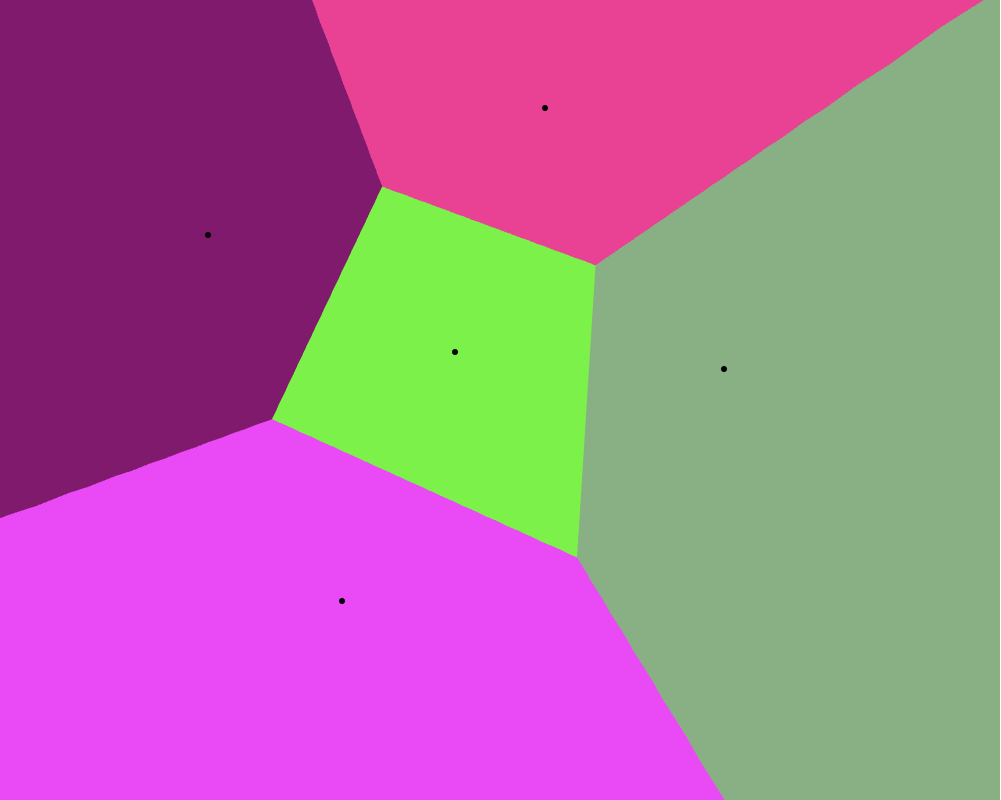
\includegraphics[scale = 0.4]{Диаграмма для задачи}
\caption{\label{tab:widgets}Пример результата работы алгоритма}

\end{figure}

\clearpage
\section{Формальная постановка задачи}
\begin{enumerate}
\item Изучить алгоритм Форчуна, описать его в форме научного доклада.
\item Реализовать версию алгоритма Форчуна с его визуализированным изображением. Это должна быть html-страница с визуальным отображением результата работы алгоритма. При заходе на нее должны отображаться изначально заданные 5 точек и диаграмма, построенная по ним. Должен присутствовать список тестовых фигур в виде интерактивных кнопок, при нажатии на которые, отображается соответствующая фигура/рисунок. Также, должна присутствовать кнопка сброса картинки. 
		  Формат выходного файла: html-страница, которая содержит диаграмму Вороного.
\item Исследовать алгоритм на предельно допустимое количество входных данных.
\item Результаты работы выложить на гитхаб.
\end{enumerate}

\newpage
ВЫВОД ИЗ ИССЛЕДОВАНИЯ

\section{Тестирование и исследование}
\subsection{Тесты}
В рамках работы была исследована производительность данного алгоритма.  Были проведены тесты по двум направлениям: по затраченному времени и по количеству потребляемых ресурсов памяти. Исследование проводилось на пяти разных по количеству наборах произвольно взятых точек: 10, 100, 1000, 10000 и 20000, соответственно.\\
\bigskip
\\Существует три типа файлов: in, out, ans.
\bigskip
\\IN - файл из которого вводятся данные.\\
OUT - файл в который выводятся данные.\\
ANS - файл с правильным ответом.\\
\bigskip
\\Формат входных данных:\\
Построчно вводятся координаты (x, y) точек.\\
\\Например:\\
13 6\\
12 10\\
8 7\\
7 3\\
3 11\\
\bigskip
\\Формат выходных данных:\\
Открывается html-страница, на которой визуально отображается рельтат работы алгоритма.



\begin{figure}[H]
\centering
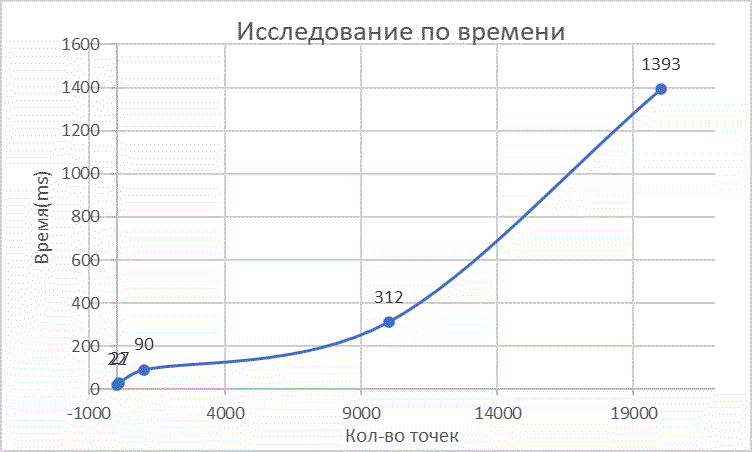
\includegraphics[scale=0.9]{time}
\caption{\label{tab:widgets}Время работы алгоритма}
\bigskip
\bigskip
\bigskip
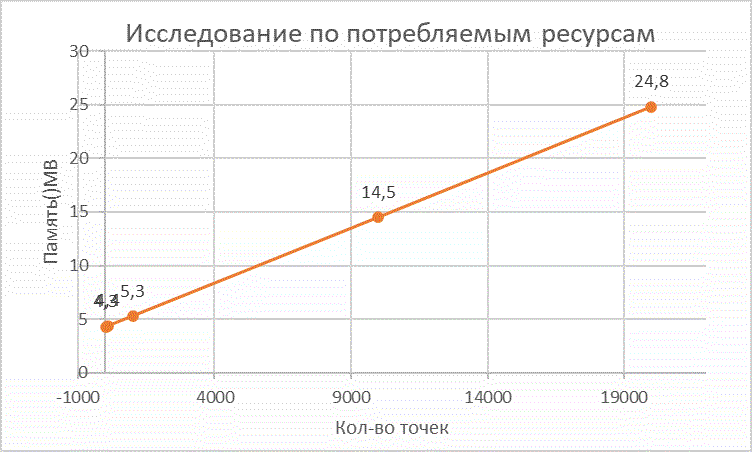
\includegraphics[scale=0.9]{resource}
\caption{\label{tab:widgets}Затрачиваемый ресурс памяти}

\end{figure}
\subsection{Результаты исследования}
Выше представлены графики O(n log n) и O(n) соответственно. Это соответствует изначальному теоретическом расчету.


\clearpage
\section{Список литературы}
\begin{enumerate}
\item Steven Fortune. A sweepline algorithm for Voronoi diagrams // ACM Digital Library Proceedings of the second annual symposium on Computational geometry. — Yorktown Heights, New York, United States, 1986. — ISBN 0-89791-194-6. 
\item Mark de Berg, Marc van Kreveld, Mark Overmars, Otfried Schwarzkopf. Computational Geometry. — 2nd revised. — Springer-Verlag, 2000. — ISBN 3-540-65620-0.
\item David Austin. Voronoi Diagrams and a Day at the Beach. — American Mathematical Society.
\item Rene Descartes, Le Monde, ou Traité de la lumière, Translation and introduction by M.S. Mahoney, Abaris, 1979.
\item A. Okabe, B. Boots, K. Sugihara, S. Chiu, Spatial Tesselations, Concepts and Applications of Voronoi Diagrams, Wiley, 2000.
\item J. O'Rourke, Computational Geometry in C, Cambridge University Press, 2000.
\item Spatial: диаграмма Вороного (Java) [Электронный ресурс] — Режим доступа: http://obi2ru.blogspot.com/2012/12/spatial-voronoi-diagram-by-java.html
\item Kenny Wong, Hausi A. Müller, An Efficient Implementation of Fortune's Plane-Sweep Algorithm for Voronoi Diagrams, CiteSeerX   10.1.1.83.5571 .
\item Wikipedia: Алгоритм Форчуна 
\item Javascript Implementation of Steven J. Fortune's Algorythm to compute Voronoi diagrams [Электронный ресус] — Режим доступа: http://www.raymondhill.net/voronoi/rhill-voronoi.html
\item Алгоритм Форчуна, подробности реализации [Электронный ресус] — Режим доступа: https://habr.com/ru/post/430628/
\item Ход «Voronoi» [Электронный ресус] — Режим доступа: https://habr.com/ru/post/110790/
\item Ход «Voronoi». Часть 2 — Бинарное дерево  [Электронный ресус] — Режим доступа: https://habr.com/ru/post/112581/
\item С++ для начинающих. Бинарное дерево. Первое знакомство [Электронный ресус] — Режим доступа: https://ci-plus-plus-snachala.ru/?p=89
\item Практика метапрограммирования на C++: бинарное дерево поиска на этапе компиляции [Электронный ресус] — Режим доступа: https://habr.com/ru/p ost/320686/
\item Fortune's Algorithm in C++ [Электронный ресус] — Режим доступа: https://www.cs.hmc.edu/-mbrubeck/voronoi.html
\item Voronoi diagrams with Fortune's algorithm  [Электронный ресус] — Режим доступа: https://www.bitbanging.space/posts/voronoi-diagram-with-fortunes-algorithm
\item Wikipedia: Fortune's algorithm
\item Fortune's algorithm  [Электронный ресус] — Режим доступа: https://wikimili.com/en/Fortune's-algorithm
\item Диаграмма Вороного и её применения [Электронный ресус] — Режим доступа: https://itnan.ru/post.php?c=1&p=309252
\item Voronoi Diagrams and a Day at the Beach [Электронный ресус] — Режим доступа: https://www.ams.org/publicoutreach/feature-column/fcarc-voronoi
\item Voronoi diagram in AS3 [Электронный ресус] — Режим доступа: https://blog.ivank.net/voronoi-diagram-in-as3.html
\item Алгоритм Форчуна на C++ для построения диаграммы Вороного на плоскости [Электронный ресус] — Режим доступа: https://www.pvsm.ru/matematika/211589
\item THE BOOST.POLYGON VORONOI LIBRARY [Электронный ресус] — Режим доступа: https://www.boost.org/doc/libs/1-52-0/libs/polygon/doc/voronoi-main.htm
\item Voronoi Diagram using Fortune's Algorithm [Электронный ресус] — Режим доступа: https://www.youtube.com/watch?v=dgEt9Go7GvE
\item Voronoi Diagrams and Procedural Map Generation [Электронный ресус] — Режим доступа: https://www.youtube.com/watch?v=3G5d8ob-Lfo
\item Fortune's Algorithm: The Details [Электронный ресус] — Режим доступа: https://pvigier.github.io/2018/11/18/fortune-algorithm-details.html
\end{enumerate}

\end{document}
